\documentclass[11pt,a4paper]{report}
\usepackage[utf8]{inputenc}
\usepackage{amsmath}
\usepackage{graphicx, xcolor}
\usepackage{tabularx}
\usepackage{adjustbox}
\usepackage{tikz, lipsum, lmodern}
\usepackage[most]{tcolorbox}

%\usepackage[colorinlistoftodos]{todonotes}
\usepackage{csquotes}
\usepackage{comment}
\usepackage{imakeidx}
\usepackage[english]{babel}

\usepackage{multicol}
\setlength{\columnsep}{1cm}

%tabella
\usepackage{multirow}
\usepackage{tcolorbox}
\usepackage[margin=3cm]{geometry}
\usepackage[hidelinks]{hyperref}
\usepackage[toc,acronym,nopostdot,nonumberlist]{glossaries}
\usepackage{titling}
\usepackage{tikzpagenodes}
\usepackage[ddmmyyyy]{datetime}
\usepackage{setspace}
\usepackage{indentfirst}

%para definir a localização das tabelas e imagens em modo strict
%\usepackage{placeins}

\usepackage{biblatex}
\addbibresource{ref.bib}
\makeglossaries

%colocar aqui variáveis que serão utilizadas no texto:
\newcommand\kbps{\text{\textit{k}bit/s}}
\doublespacing

\begin{document}
\begin{titlepage}
\begin{tikzpicture}[remember picture,overlay,shift={(current page.center)}]
\node[anchor=center,xshift=-3cm,yshift=9cm]{
\includegraphics[scale=0.25]{figs/MCiber-logo.pdf}};
\node[anchor=center,xshift=3cm,yshift=8.3cm]{
\includegraphics[scale=0.65]{figs/letter-MCiber.pdf}};
\node[anchor=center,xshift=7cm,yshift=-12cm]{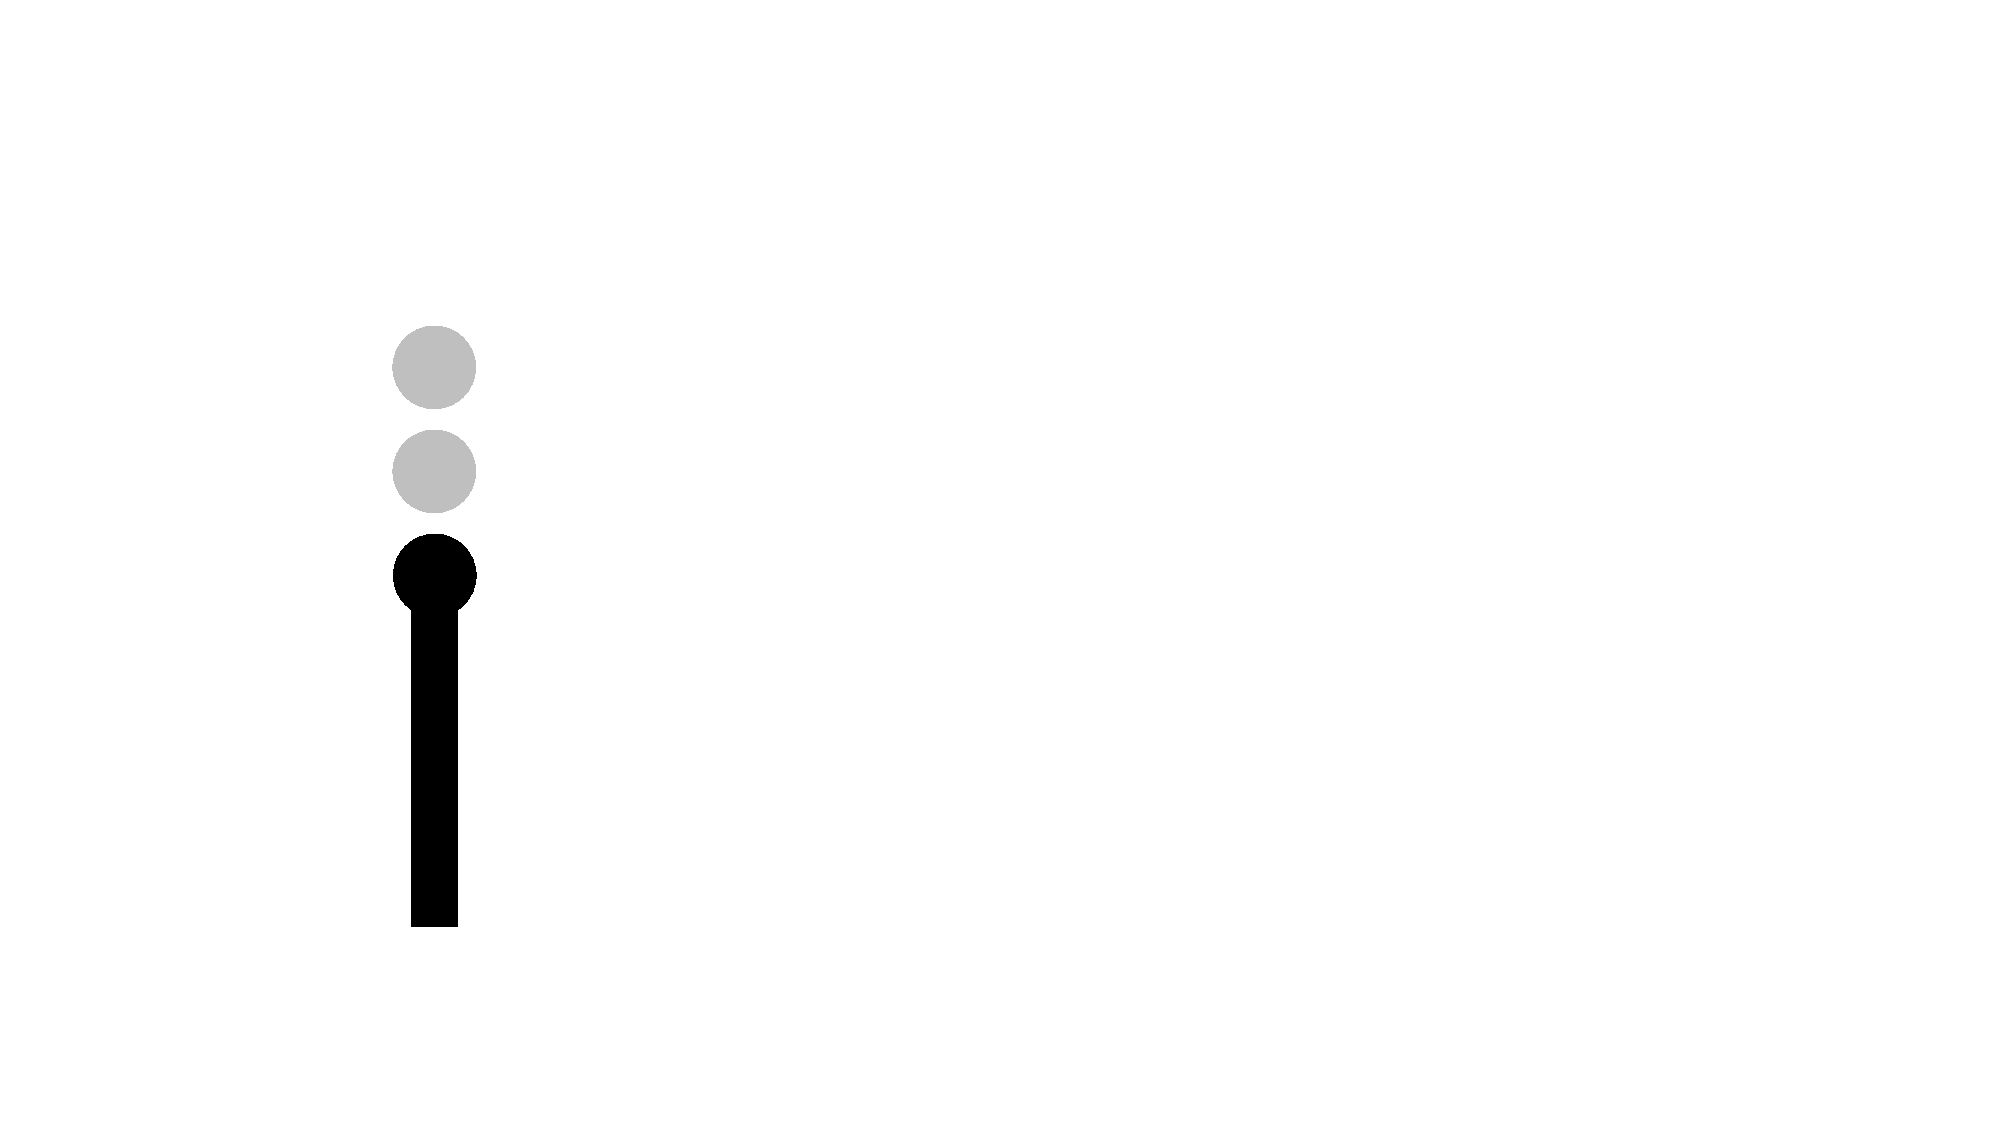
\includegraphics[scale=0.7]{figs/MCiber-end2.pdf}};
\end{tikzpicture}

\centering
\vspace{7cm}
\huge Title of the Project\\
\vspace{2cm}
\large a Thesis authored by\\
%\large a lab assignment report authored by\\
\Large Name of the student\\
\vspace{3cm}
\large supervised by\\
\large Prof. X and Prof. Y\\
\vspace{2cm}
\newdateformat{daymonthyear}{\THEDAY\ \monthname[\THEMONTH], \THEYEAR}
\daymonthyear\today \\
\vspace{1cm}

\includegraphics[scale=0.4]{figs/ESTG-logo.png}
%December, 2019
%\large v2.3
\end{titlepage}

%%%% colocar aqui acrónimos
\newacronym{mcyber}{MCyber}{Master in Cybersecurity}
\newacronym{wn}{WN}{Wireless Network}

%%%%%%%%%%%%%%%%%%%%%%%%%%%%%%%%%%%%%%%%%%%%%%%%%%%%%
\begin{abstract}
context
The quick brown fox jumps over the lazy dog. The quick brown fox jumps over the lazy dog. The quick brown fox jumps over the lazy dog. The quick brown fox jumps over the lazy dog. The quick brown fox jumps over the lazy dog. The quick brown fox jumps over the lazy dog.

\end{abstract}


\textbf{Keywords:} word1. word2. word3. word4.

%insert index
\tableofcontents
\glsaddall
\printglossary[type=\acronymtype]
\printglossary[type=main,title={Glossary},toctitle={Glossary}]
%%%%%%%%%%%%%%%%%%%%%%%%%%%%%%%%%%%%%%%%%%%%%%%%%%%%%

\chapter{Introduction}
\label{chap:introduction}

In this Chapter ...

IMPORTANT:
\begin{itemize}
    \item PLEASE check the file vars.tex: I'm using it in 10\kbps.
    \item Using glossaries for the first time: \gls{wn}
    \item Using glossaries after first time: \gls{wn}
    \item Using glossaries in plural: \glspl{wn}
    \item Using glossaries extended: \glsdesc{wn}
\end{itemize}

How to reference and insert a figure \ref{fig:labeloffigure}.

\begin{figure}[ht]
    \centering
    
\includegraphics[scale=0.2]{figs/MCiber-logo.pdf}
    \caption{This is a figure}
    \label{fig:labeloffigure}
\end{figure}

This is an example of a citation \cite{Pedro2019}.

This is a way for you to generate tables:

https://www.tablesgenerator.com/

The quick brown fox jumps over the lazy dog. The quick brown fox jumps over the lazy dog. The quick brown fox jumps over the lazy dog. The quick brown fox jumps over the lazy dog. The quick brown fox jumps over the lazy dog. The quick brown fox jumps over the lazy dog.

\section{Context}
\label{sec:context}
%Context
The quick brown fox jumps over the lazy dog. The quick brown fox jumps over the lazy dog. The quick brown fox jumps over the lazy dog. The quick brown fox jumps over the lazy dog. The quick brown fox jumps over the lazy dog. The quick brown fox jumps over the lazy dog.

\begin{tcolorbox}[colback=yellow!10!white,colframe=red!75!black,%lowerbox=invisible,
  savelowerto=\jobname_ex.tex]
  Now, we play hide and seek. Where is the lower part?
  \tcblower
  I'm invisible until you find me.
\end{tcolorbox}

%context focus
The quick brown fox jumps over the lazy dog. The quick brown fox jumps over the lazy dog. The quick brown fox jumps over the lazy dog. 

\begin{equation}
	x_{1,2}=\frac{-b\pm\sqrt{b^2-4ac}}{2a}
\end{equation}

The quick brown fox jumps over the lazy dog.
The quick brown fox jumps over the lazy dog. The quick brown fox jumps over the lazy dog.

\begin{equation}
	(x+3)(x+2)=x^2+5x+6\notag\\
	\geq x^2
\end{equation}
\begin{gather}
	(x+3)(x+2)=x^2+5x+6\notag\\
	\geq x^2
\end{gather}
\begin{align}
	(x+3)(x+2)&=x^2+5x+6\notag\\
	&\geq x^2
\end{align}

\section{Problem Statement and Motivation}
\label{sec:motivation}

%problem to solve
The quick brown fox jumps over the lazy dog. The quick brown fox jumps over the lazy dog. The quick brown fox jumps over the lazy dog.\\
\begin{tcolorbox}
\newtcolorbox{mybox}{colback=red!5!white,colframe=red!75!black}
A physical explanation the \emph{dynamic matrix}\\
The motivation of the current project is
The quick brown fox jumps over the lazy dog. The quick brown fox jumps over the lazy dog. The quick brown fox jumps over the lazy dog. The quick brown fox jumps over the lazy dog. The quick brown fox jumps over the lazy dog. The quick brown fox jumps over the lazy dog.\\
\end{tcolorbox}
The quick brown fox jumps over the lazy dog. The quick brown fox jumps over the lazy dog. The quick brown fox jumps over the lazy dog.\\

\begin{tcolorbox}
A physical explanation the 
\emph{dynamic matrix}\\
The motivation of the current project is
The quick brown fox jumps over the lazy dog. The quick brown fox jumps over the lazy dog. The quick brown fox jumps over the lazy dog. The quick brown fox jumps over the lazy dog. The quick brown fox jumps over the lazy dog. The quick brown fox jumps over the lazy dog.
\end{tcolorbox}

%point the motivation
The motivation of the current project is The quick brown fox jumps over the lazy dog. The quick brown fox jumps over the lazy dog. The quick brown fox jumps over the lazy dog. The quick brown fox jumps over the lazy dog. The quick brown fox jumps over the lazy dog. The quick brown fox jumps over the lazy dog.\\

\begin{multicols}{2}

\section{First Section}
\noindent
All human things are subject to decay. And when fate summons, Monarchs must obey.\\

Hello, here is some text without a meaning. This text should show what a printed text will look like at this place. If you read this text, you will get no information. Really?  Is there 
no information?  Is there...\\ 
The quick brown fox jumps over the lazy dog. The quick brown fox jumps over the lazy dog. The quick brown fox jumps over the lazy dog. The quick brown fox jumps over the lazy dog. The quick brown fox jumps over the lazy dog. The quick brown fox jumps over the lazy dog.\\ 
The quick brown fox jumps over the lazy dog. The quick brown fox jumps over the lazy dog. The quick brown fox jumps over the lazy dog. The quick brown fox jumps over the lazy dog. The quick brown fox jumps over the lazy dog. The quick brown fox jumps over the lazy dog.
\end{multicols}

\section{Objectives}
\label{sec:name}
The general objective is to
The quick brown fox jumps over the lazy dog. The quick brown fox jumps over the lazy dog. The quick brown fox jumps over the lazy dog.\\

\begin{tcolorbox}
Here is some text
\end{tcolorbox}

\begin{tcolorbox}[width=5cm]
Here is some text
\end{tcolorbox}

\begin{tcolorbox}[width=.5\textwidth, colframe=red]
Here is some text
\end{tcolorbox}

\begin{tcolorbox}[width=8cm, colframe=red, colback=blue!30, halign=right]
Here is some text
\end{tcolorbox}

\begin{tcolorbox}[width=.5\linewidth, halign=center, colframe=red, colback=blue!30, boxsep=5mm, arc=3mm]
Here is some text
\end{tcolorbox}

\begin{tcolorbox}[width=7cm, colframe=red, colback=blue!30, arc=3mm, sharp corners=east]
Here is some text
\end{tcolorbox}

The quick brown fox jumps over the lazy dog. The quick brown fox jumps over the lazy dog. The quick brown fox jumps over the lazy dog.

\section{Organization}
\label{sec:org}
The quick brown fox jumps over the lazy dog. The quick brown fox jumps over the lazy dog. The quick brown fox jumps over the lazy dog. The quick brown fox jumps over the lazy dog. The quick brown fox jumps over the lazy dog. The quick brown fox jumps over the lazy dog.

\chapter{Title of the chapter}
\label{cap:name1}

The quick brown fox jumps over the lazy dog.\\
\colorbox{pink}{\parbox{\textwidth}{%
  \vskip10pt
  \leftskip10pt\rightskip10pt
  \lipsum[1]
  \vskip10pt
 }

The quick brown fox jumps over the lazy dog. The quick brown fox jumps over the lazy dog. The quick brown fox jumps over the lazy dog. The quick brown fox jumps over the lazy dog. The quick brown fox jumps over the lazy dog.

\section{Section 1}
\label{sec:sec1}
\noindent
The quick brown fox jumps over the lazy dog. The quick brown fox jumps over the lazy dog. The quick brown fox jumps over the lazy dog. The quick brown fox jumps over the lazy dog. The quick brown fox jumps over the lazy dog. The quick brown fox jumps over the lazy dog.

\setlength{\parindent}{0pt}
\setlength{\parskip}{1em}
\renewcommand{\baselinestretch}{2.0}

This is the first paragraph, contains some text to test the paragraph
interlining, paragraph indentation and some other features. Also, is 
easy to see how new paragraphs are defined by simply entering a double 
blank space.

\colorbox{pink}{\hbox to \textwidth{alert box\hfill}}

\textcolor{brown}{Hello, here is some text without a meaning.}

\colorbox{pink}{\parbox{\textwidth}{\lipsum[1]}}

Hello, here is some text without a meaning. This text should
show what a printed text will look like at this... 

\begin{itemize}
    \item The quick brown fox jumps over the lazy dog. The quick brown fox jumps over the lazy dog. The quick brown fox jumps over the lazy dog. The quick brown fox jumps over the lazy dog. The quick brown fox jumps over the lazy dog. The quick brown fox jumps over the lazy dog.
    \item The quick brown fox jumps over the lazy dog. The quick brown fox jumps over the lazy dog. The quick brown fox jumps over the lazy dog. The quick brown fox jumps over the lazy dog. The quick brown fox jumps over the lazy dog. The quick brown fox jumps over the lazy dog.
\end{itemize}\\

%-----------------------color box
\section{Colored boxes}

\begin{tcolorbox}[colback=red!5!white,colframe=red!75!black]
  My box.
\end{tcolorbox}

\begin{tcolorbox}[colback=blue!5!white,colframe=blue!75!black,title=My title]
  My box with my title.
\end{tcolorbox}

\begin{tcolorbox}[colback=green!5!white,colframe=green!75!black]
  Upper part of my box.
  \tcblower
  Lower part of my box.
\end{tcolorbox}

\begin{tcolorbox}[colback=yellow!5!white,colframe=yellow!50!black,
  colbacktitle=yellow!75!black,title=My title]
  I can do this also with a title.
  \tcblower
  Lower part of my box.
\end{tcolorbox}

\begin{tcolorbox}[colback=yellow!10!white,colframe=red!75!black,lowerbox=invisible,
  savelowerto=\jobname_ex.tex]
  Now, we play hide and seek. Where is the lower part?
  \tcblower
  I'm invisible until you find me.
\end{tcolorbox}

\begin{tcolorbox}[colback=yellow!10!white,colframe=red!75!black,title=Here I am]
  \input{\jobname_ex.tex}
\end{tcolorbox}


\begin{tcolorbox}[enhanced,sharp corners=uphill,
    colback=blue!50!white,colframe=blue!25!black,coltext=yellow,
    fontupper=\Large\bfseries,arc=6mm,boxrule=2mm,boxsep=5mm,
    borderline={0.3mm}{0.3mm}{white}]
  Funny settings.
\end{tcolorbox}


\begin{tcolorbox}[enhanced,frame style image=blueshade.png,
  opacityback=0.75,opacitybacktitle=0.25,
  colback=blue!5!white,colframe=blue!75!black,
  title=My title]
  This box is filled with an external image.\par
  Title and interior are made partly transparent to show the image.
\end{tcolorbox}


\begin{tcolorbox}[enhanced,attach boxed title to top center={yshift=-3mm,yshifttext=-1mm},
  colback=blue!5!white,colframe=blue!75!black,colbacktitle=red!80!black,
  title=My title,fonttitle=\bfseries,
  boxed title style={size=small,colframe=red!50!black} ]
  This box uses a \textit{boxed title}. The box of the title can
  be formatted independently from the main box.
\end{tcolorbox}


\clearpage
%----------------------------------------------------------
\section{\LaTeX-Examples}

\begin{tcblisting}{colback=red!5!white,colframe=red!75!black}
This is a \LaTeX\ example:
\begin{equation}
\sum\limits_{i=1}^n i = \frac{n(n+1)}{2}.
\end{equation}
\end{tcblisting}


\begin{tcblisting}{colback=red!5!white,colframe=red!75!black,listing side text,
  title=Side by side,fonttitle=\bfseries}
This is a \LaTeX\ example:
\begin{equation}
\sum\limits_{i=1}^n i = \frac{n(n+1)}{2}.
\end{equation}
\end{tcblisting}


%----------------------------------------------------------
\section{Theorems}

\newtcbtheorem[auto counter,number within=section]{theo}%
  {Theorem}{fonttitle=\bfseries\upshape, fontupper=\slshape,
     arc=0mm, colback=blue!5!white,colframe=blue!75!black}{theorem}

\begin{theo}{Summation of Numbers}{summation}
  For all natural number $n$ it holds:
  \begin{equation}
  \tcbhighmath{\sum\limits_{i=1}^n i = \frac{n(n+1)}{2}.}
  \end{equation}
\end{theo}

We have given Theorem \ref{theorem:summation} on page \pageref{theorem:summation}.

\newtcbtheorem[use counter from=theo]{antheo}%
  {Theorem}{theorem style=change,oversize,enlarge top by=1mm,enlarge bottom by=1mm,
    enhanced jigsaw,interior hidden,fuzzy halo=1mm with green,
     fonttitle=\bfseries\upshape,fontupper=\slshape,
     colframe=green!75!black,coltitle=green!50!blue!75!black}{antheorem}

\begin{antheo}{Summation of Numbers}{summation}
  For all natural number $n$ it holds:
  \begin{equation}
  \tcbhighmath{\sum\limits_{i=1}^n i = \frac{n(n+1)}{2}.}
  \end{equation}
\end{antheo}

%----------------------------------------------------------
\section{Watermarks}

\begin{tcolorbox}[enhanced,watermark graphics=Basilica_5.png,
  watermark opacity=0.3,watermark zoom=0.9,
  colback=green!5!white,colframe=green!75!black,
  fonttitle=\bfseries, title=Box with a watermark picture]
  Here, you see my nice box with a picture as a watermark.
  This picture is automatically resized to fit the dimensions
  of my box. Instead of a picure, some text could be used or
  arbitrary graphical code. See the documentation for more options.
\end{tcolorbox}

%----------------------------------------------------------
\section{Boxes in boxes}
\begin{tcolorbox}[colback=yellow!10!white,colframe=yellow!50!black,
  every box/.style={fonttitle=\bfseries},title=Box]
  \begin{tcolorbox}[enhanced,colback=red!10!white,colframe=red!50!black,
    colbacktitle=red!85!black,
    title=Box inside box,drop fuzzy shadow]
    \begin{tcolorbox}[beamer,colframe=blue!50!black,title=Box inside box inside box]
      And now for something completely different: Boxes!\par\medskip
      \newtcbox{\mybox}[1][]{nobeforeafter,tcbox raise base,colframe=green!50!black,colback=green!10!white,
        sharp corners,top=1pt,bottom=1pt,before upper=\strut,#1}
      \mybox[rounded corners=west]{This} \mybox{is} \mybox{another} \mybox[rounded corners=east]{box.}
    \end{tcolorbox}
  \end{tcolorbox}
\end{tcolorbox}

%----------------------------------------------------------
\section{Breakable Boxes}
\begin{tcolorbox}[enhanced jigsaw,breakable,pad at break*=1mm,
  colback=blue!5!white,colframe=blue!75!black,title=Breakable box,
  watermark color=white,watermark text=\Roman{tcbbreakpart}]
  \lipsum[1-12]
\end{tcolorbox}

%----------------------------------------------------------
\clearpage
\section{Fit Boxes}

\begin{tcolorbox}[enhanced,fit to height=10cm,
  colback=green!25!black!10!white,colframe=green!75!black,title=Fit box (10cm),
  drop fuzzy shadow,watermark color=white,watermark text=Fit]
  \lipsum[1-4]
\end{tcolorbox}

\begin{tcolorbox}[enhanced,fit to height=5cm,
  colback=green!25!black!10!white,colframe=green!75!black,title=Fit box (5cm),
  drop fuzzy shadow,watermark color=white,watermark text=Fit]
  \lipsum[1-4]
\end{tcolorbox}

%%%%%%%%%%%%%%%%%%%%%%%%%%%%%%%%%%%%%%%%%%%%%%%%%%%%%
\chapter{Title of the chapter}
\label{cap:name2}

The quick brown fox jumps over the lazy dog. The quick brown fox jumps over the lazy dog. The quick brown fox jumps over the lazy dog. The quick brown fox jumps over the lazy dog. The quick brown fox jumps over the lazy dog. The quick brown fox jumps over the lazy dog.\\

\begin{tcolorbox}
\newtcolorbox{mybox}{colback=red!5!white,colframe=red!75!black}
A physical explanation the \emph{dynamic matrix}\\
lots of text\\
a new line\\
equation
\begin{equation}
    %\label{eq:dynamic_diag}
    \nonumber
        \bm C \bm D \bm C^{\dagger}=\bm \Omega = \left(\begin{array}{cccc}
            \omega^2_1 & 0 & ... & 0\\
            0 & \omega^2_2 & ... & 0\\
            \vdots &  & \ddots & \vdots \\
            0 & 0 & ... & \omega^2_{Nd}
        \end{array}\right),
\end{equation}
where $\bm C$ is a unitary matrix (each column is one of the eigenvectors of the dynamic matrix $\bm D$), $Nd$ is the product of the number of particlces, $N$, and the number of dimensions, $d$.
\end{tcolorbox}

\section{Section 2}
\label{sec:sec2}

The quick brown fox jumps over the lazy dog. The quick brown fox jumps over the lazy dog. The quick brown fox jumps over the lazy dog. The quick brown fox jumps over the lazy dog. The quick brown fox jumps over the lazy dog. The quick brown fox jumps over the lazy dog.


\addcontentsline{toc}{chapter}{References}
\printbibliography[title={References}]

\end{document}
